\section{Introduction}

The generators that supply electricity to our homes and the motors in our cars
are important devices whose mechanism of operation is typically taken for 
granted. Today, we'll explore the fundamental physical law responsible for 
their operation, Faraday's law of induction.

Faraday's law states that a changing magnetic field can produce an induced 
voltage in an electric circuit.  The device we will study is a simple
transformer, two coils of wire linked by an iron core.  It operates by
running an alternating current (the input) through one coil (the primary coil)
to generate an alternating magnetic field in the iron. (This phenomenon is 
described by another fundamental law, called Amp\`{e}re's law.)  The magnetic 
field passes through the second coil (the secondary coil), where, by Faraday's 
law, it induces an alternating potential (the output) across the coil. This 
voltage can be viewed on the oscilloscope (remember that it's varying in time),
so that its properties can be studied.

In particular, we will examine the output signal from the transformer when we
use a sinusoidal input. We will see that the output is also sinusoidal and we
will examine the dependence of the output amplitude on both the frequency of
the input signal and the number of turns in the secondary coil. We will also
examine the output for other input signals: triangle waves and square waves.
Examining these signals will reveal that the output signals is proportional
to the {\it time derivative} of the input signal.

\vfill
\pagebreak

\section{Theory}

\subsection{References}

Faraday's law of induction is introduced in Serway, Chapter~31 (Faraday's
Law).  Chapter~33 (Alternating Current Circuits) is also 
useful, since we're using AC circuits.  The magnetic field of a solenoid is 
discussed in Sections~30.4 (The Magnetic Field of a Solenoid), and~30.5
(The Magnetic Field Along the Axis of a Solenoid).

\subsection{Magnetic Flux}

Whenever we have a vector field present we may speak of the flux of that field 
through a surface.  If we have a magnetic field $\vec{B}$ which passes through 
an open surface $S$ as in Figure~\ref{fig:ind:fluxdef},
\begin{figure}[htb]
\centering 
\epsfxsize=7cm 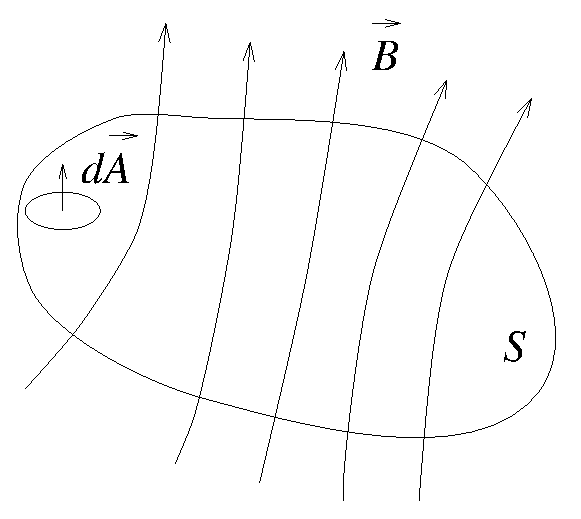
\includegraphics[scale=0.6]{6_induction/fluxdef.eps}
\caption{A magnetic flux $\Phi_M$ passes through the surface $S$.}
\label{fig:ind:fluxdef}
\end{figure}
then we define the magnetic flux to be the integral
$$
\Phi_M=\int_S \vec{B}\cdot d\vec{A},
$$
where $d\vec{A}$ is the perpendicularly oriented differential area element.

Let's calculate the magnetic flux which passes through a long thin solenoid, 
of $N$ turns, length $L$, radius $a\ll L$, and carrying a current $I$, 
illustrated in Figure~\ref{fig:ind:solenoid}. 
\begin{figure}[htb]
\centering 
\epsfxsize=9cm 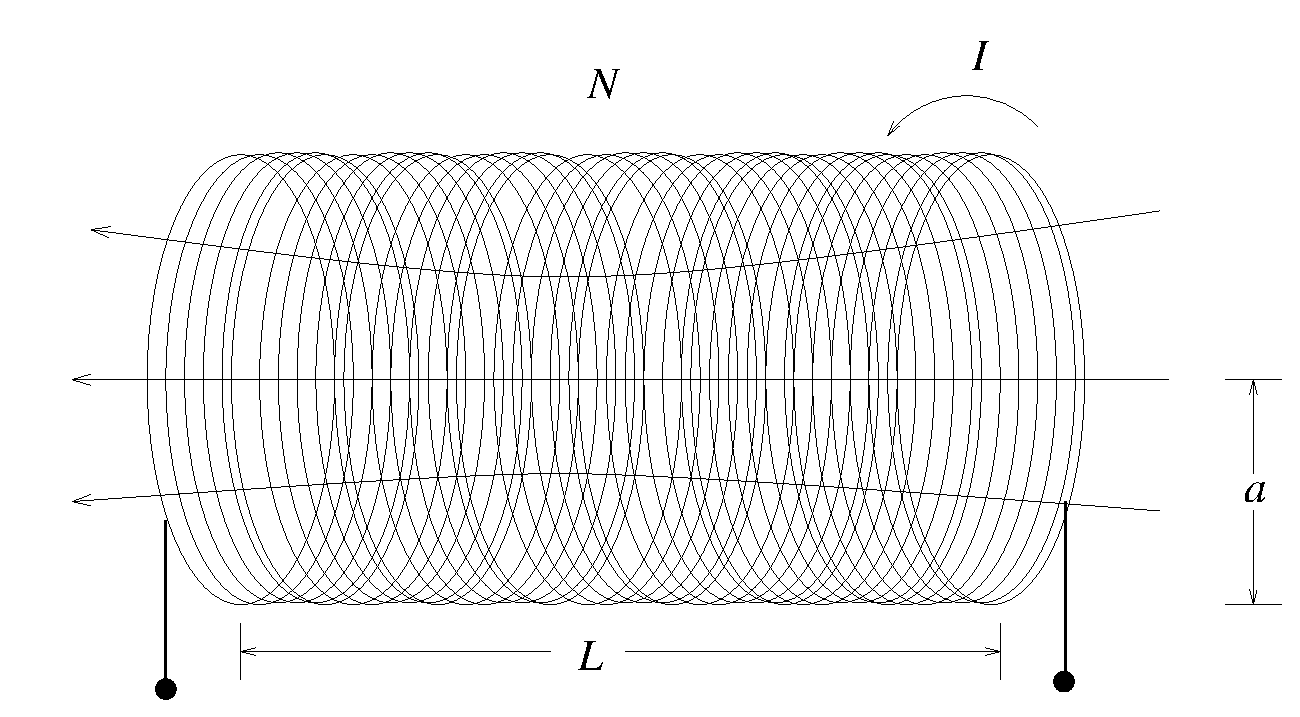
\includegraphics[scale=0.6]{6_induction/solenoid.eps}
\caption{A long thin solenoid (not to scale).}
\label{fig:ind:solenoid}
\end{figure}
We'll consider the field responsible for the flux to be that of the solenoid 
itself, so this is an example of {\it self-induction}. The magnetic field 
along the cross section of the solenoid is roughly constant and given by
$$ B= \frac{\mu_0 N I}{L}; $$
for a more complete discussion, see Serway. The flux is then
\begin{eqnarray}
\Phi_M &=& \int_S \vec{B}\cdot d\vec{A} \nonumber \\
&=& \int_0^{2\pi} d\theta \int_0^a r dr \frac{\mu_0 NI}{L} \nonumber \\
&=& \frac{\mu_0 NI}{L} (\pi a^2) \nonumber \\
\Phi_M &=& \frac{\pi\mu_0N Ia^2}{L} \label{eq:ind:fluxgen}
\end{eqnarray}

\subsection{Faraday's Law}

Consider again the solenoid in Figure~\ref{fig:ind:solenoid}, but this time 
imagine that the magnetic field is time-varying and is coming from some
external source, perhaps another coil, rather than from a current running 
through the solenoid.  Faraday's law states that the magnetic flux through the 
solenoid induces a voltage
\begin{equation}
V=-N\frac{d\Phi_M}{dt} \label{eq:ind:faraday}
\end{equation}
across the solenoid.  The factor of $N$ appears because the flux $\Phi_M$ links
each of the $N$ coils of the solenoid; the voltages induced by $\Phi_M$ in 
each turn of the coil add in series. 

\subsection{The Transformer}

Let's now apply what we've learned to a transformer, illustrated in 
Figure~\ref{fig:ind:transformer}. 
\begin{figure}[htb]
\centering 
\epsfxsize=10cm 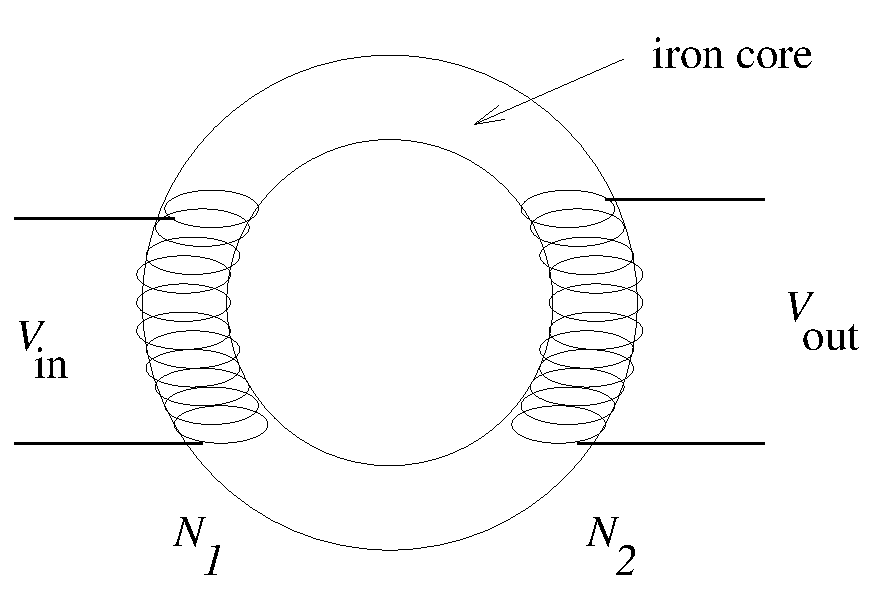
\includegraphics[scale=0.6]{6_induction/transformer.eps}
\caption{A simple transformer.}
\label{fig:ind:transformer}
\end{figure}
A voltage $V_{\rm{in}}$ is supplied to a primary coil of $N_1$ turns,
producing a current $I_{\rm{in}}$, which, from~(\ref{eq:ind:fluxgen}),
generates a flux 
$$\Phi= \frac{\pi\mu  N_1 a_1^2}{L_1} I_{\rm{in}},
$$
in the iron core. We assume that, since the iron is a magnetic material, it
holds this flux and carries it through the secondary coil of $N_2$ turns;
since we aren't dealing with a field in vacuo anymore, we have replaced 
$\mu_0$ by $\mu$, the permeability of iron. 
Faraday's law~(\ref{eq:ind:faraday}) implies that a voltage, given by 
$$V_{\rm{out}} = - N_2\frac{d\Phi}{dt},$$  
is generated across the secondary coil.  We can substitute in for $\Phi$ to 
write
$$
V_{\rm{out}} = - \left( \frac{\pi\mu  N_1 a_1^2}{L_1} \right) N_2 
\frac{d I_{\rm{in}}}{dt}.
$$
Now, in our experimental setup, we will vary $N_2$ and $I_{\rm{in}}$, but 
will not vary or measure $a_1,L_1$, or $N_1$. It will therefore be useful to 
define the (positive) constant $C'=\pi\mu  N_1 a_1^2/L_1$ and write
\begin{equation}
\fbox{$ \displaystyle V_{\rm{out}}= -C' N_2 \frac{d I_{\rm{in}}}{dt}$}, \label{eq:ind:transformer}
\end{equation}
which illustrates the dependences that we will study, leaving the constant
$C'$ to conveniently sum up the (unknown, but unchanging) properties of the 
transformer.  We see that $V_{\rm{out}}$ depends linearly on $N_2$, the 
number of turns in the secondary coil, and also depends linearly on the
time derivative of $I_{\rm{in}}$.  We also note that there is an important
minus sign in~(\ref{eq:ind:transformer}) which corresponds to the minus sign
in Faraday's law~(\ref{eq:ind:faraday}). This is called Lenz's law: the induced
voltage {\it opposes} the change in flux.  
  
Let's see what the relationship~(\ref{eq:ind:transformer}) predicts for the 
output when we use a sinusoidal input current
\begin{equation}
I_{\rm{in}} = I_0 \sin\omega t. \label{eq:ind:currentin}
\end{equation}
Using (\ref{eq:ind:transformer}) yields
\begin{equation}
V_{\rm{out}}= -C' N_2 \omega I_0 \cos\omega t. \label{eq:ind:voltageout}
\end{equation}
Figure~{\ref{fig:ind:sinusoid} shows a plot of a sine wave versus the negative
of a cosine wave.
There is therefore a phase difference of $90^\circ$ (that between sine and 
--cosine) between the input current and output voltage, while the amplitude
of the latter (the part in front of the cosine function) is proportional to
the amplitude and frequency of the former, as well as the number of turns in
the secondary coil.

To confirm these predictions, we have to be able to monitor the current
through the input coil. The problem though is that an oscilloscope (the most
suitable instrument for observing a changing signal) measures voltages. To
overcome this difficulty we use a monitoring resistor, $R_{\rm{mon}}$,
connected in series with the input coil. From Ohm's law, we know that a current
$I_{\rm{in}}$ through this resistor will cause a voltage drop
$$
V_{\rm{mon}}=I_{\rm{in}}R_{\rm{mon}}
$$
across it. For a current input of the form (\ref{eq:ind:currentin}), the
oscilloscope will measure a sinusoidal voltage signal
$$
V_{\rm{mon}} = I_0 R_{\rm{mon}} \sin \omega t.
$$
We expect then the amplitudes of the input and output signals to be related by
$$
\frac{A_{\rm{out}}}{A_{\rm{in}}} = \frac{C' N_2 \omega I_0}
{I_0 R_{\rm{mon}}} = \frac{C'}{R_{\rm{mon}}} N_2 \omega
$$
or, if we absorb the constant resistance into a new $C=C'/R_{\rm{mon}}$,
\begin{equation}
\fbox{$ \displaystyle  A_{\rm{out}} = C N_2 \omega A_{\rm{in}}$}.
\end{equation}
The amplitude of the output voltage, $A_{\rm{out}}$, should therefore depend
linearly on both $N_2$ and $\omega$.
\begin{figure}[htb]
\centering 
\epsfxsize=10cm \includegraphics[scale=0.6]{6_induction/sinusoid.eps}
\caption{A plot of a sine wave and a --cosine wave.}
\label{fig:ind:sinusoid}
\end{figure}

\section{Apparatus}

The apparatus we will use centers around the transformer box, illustrated in
Figure~\ref{fig:ind:connect}, which houses a transformer such as that in 
Figure~\ref{fig:ind:transformer}, but which allows us to vary the number of 
turns in the secondary coil. 
Note that each setting of the knob corresponds to
{\it four} turns in the coil}. We will use the function generator to provide 
our input signals and the oscilloscope to view both the input and output 
signals.


\clearpage

%  Label worksheets by \thechapter.W
\renewcommand{\thesection}{\thechapter.W}

\section{Electromagnetic Induction Worksheet}

{\bf \Large Name:}~ \rule{5cm}{.1mm}~~~~~~~
{\bf \Large Day/Time:}~\rule{3cm}{.1mm}\\
{\bf \Large Partner's Name:}~\rule{6cm}{.1mm}\\
\label{sec:ind:proc}

Before doing anything else, examine the transformer box.  Turn it over so that
you can see the coils inside.  Does it resemble a transformer such as that 
we've been talking about, {\it i.e.}, that in 
Figure~\ref{fig:ind:transformer}?  Connect the box to the function generator
and oscilloscope as in Figure~\ref{fig:ind:connect}.
\begin{figure}[htb]
\centering 
\epsfxsize=12cm 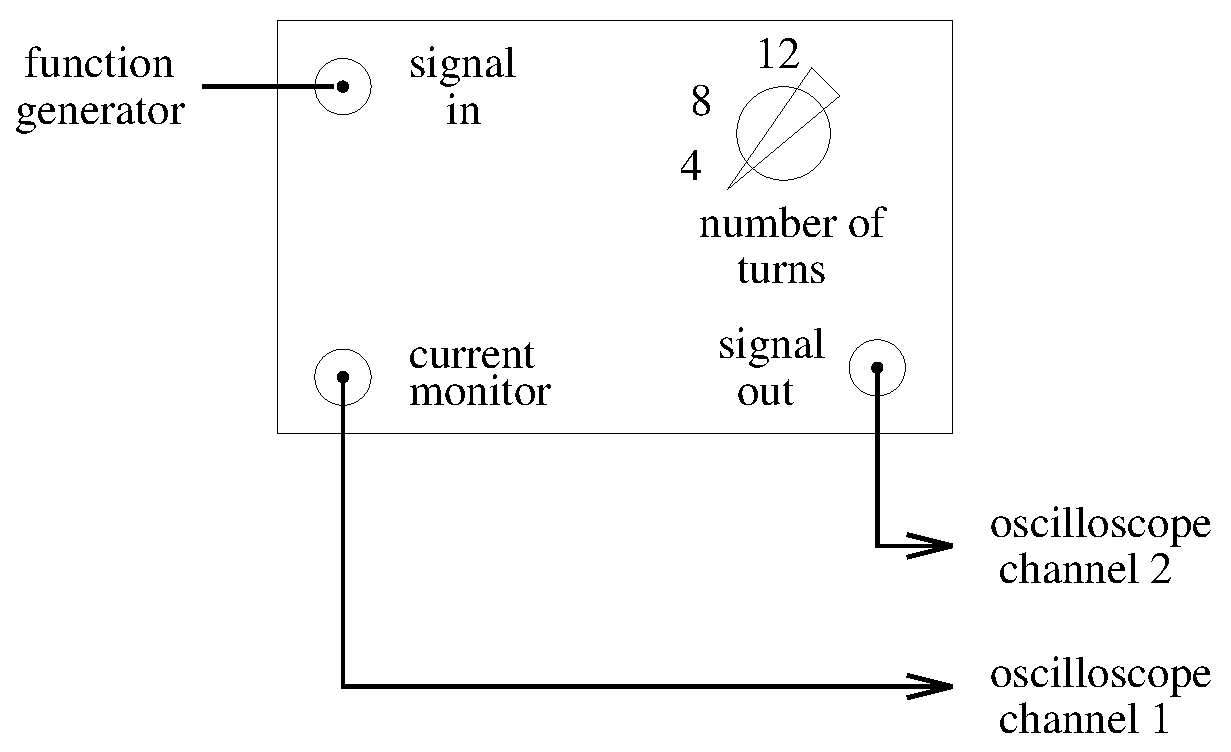
\includegraphics[scale=0.6]{6_induction/connect.eps}
\caption{How to connect the transformer box.}
\label{fig:ind:connect}
\end{figure}

\subsubsection{Sinusoidal Input}

Set the function generator to produce a good sinusoidal signal. You may need
to try different frequencies (use the range selector) to get an optimal
picture. Adjust the oscilloscope so that it displays both the input and output
signals. Set the channel 1 and channel 2 V/div and sec/div scales so that
the waveforms fill the screen. Compare the picture on the screen with that of
Figure~\ref{fig:ind:sinusoid}. Specifically, check the relative position of
the two waveforms, to confirm the connections and operation of your setup. 
Sketch the two waveforms on the grid below. Sketch both the input and output
on the same grid, but make sure you label each channel. Use the second grid
only if you make a mistake.  {\bf Draw carefully.}  You will be answering
questions based on this sketch in the classroom.\\
\ \\
\ \\
\begin{tabular}{ccc}
\epsfxsize=7cm 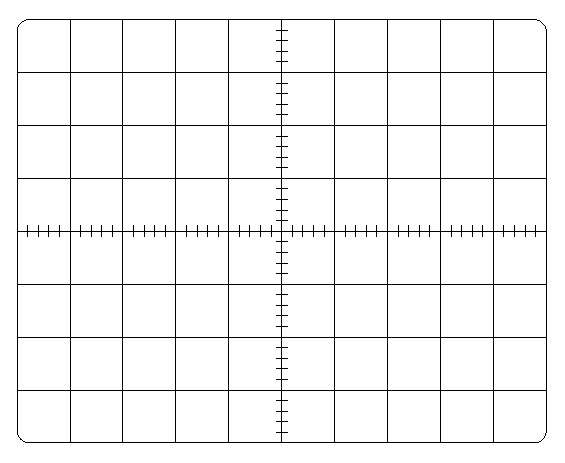
\includegraphics[scale=0.6]{6_induction/scope.eps} & \hspace{0.5cm} &
\epsfxsize=7cm 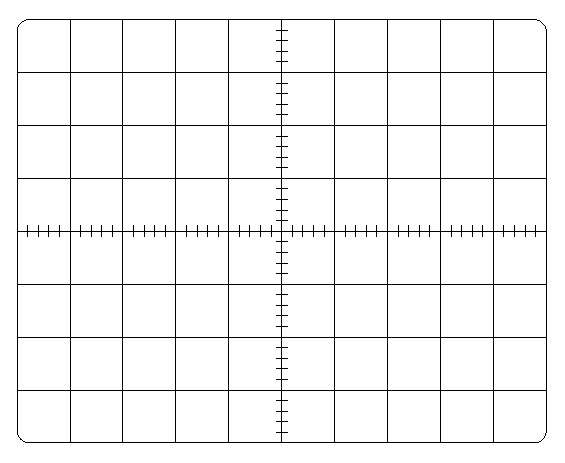
\includegraphics[scale=0.6]{6_induction/scope.eps}
\end{tabular}\\
\ \\

\noindent Measure the phase shift, %\Delta t$, between the 2 waveforms, 
(refer to $\S$~\ref{sec:SCOPE:waveprop}) and their periods, $T$. \\
\ \\
\noindent $\Delta t = $\rule{3cm}{.1mm} \\
\ \\
$T$ (ch. 1): \rule{3cm}{.1mm} \hspace*{1cm} $T$ (ch. 2): 
\rule{3cm}{.1mm} \\
\ \\

\noindent Measure the output peak-to-peak amplitude, $A_{\rm{out}}$, as
well as the current monitor signal peak-to-peak amplitude, $A_{\rm{in}}$,
and period, $T$, for 10 well spaced frequencies.
{\bf DO not go above 100kHz on the function generator.} Calculate the angular
frequency values, $\omega$, by measuring the period of the input wave on 
the oscilloscope; {\it do not} trust the frequency values read off the
function generator. {\bf Show} a sample calculation for $\omega$ and
$\Delta(\omega)$, as well as $A_{\rm{out}}/A_{\rm{in}}$ and
$\Delta(A_{\rm{out}}/A_{\rm{in}})$, here.\\
\vfill
\pagebreak

\noindent Enter your measured values of $A_{\rm{out}}$, $A_{\rm{in}}$ and
$T$ with uncertainties into Table ~\ref{tab:in:Avsw}.

\begin{table}[htb]
\begin{center}
\begin{tabular}{|c|c|c|c|c|}
\hline
\multicolumn{5}{|c|}{Amplitude versus Frequency}\\
\hline 
$A_{out}$ & $A_{in}$ & $T$ & $\omega$ & $A_{out}/A_{in}$ \\
\hline
\hspace*{2.5cm} & \hspace*{2.5cm} & \hspace*{2.5cm} & \hspace*{2.5cm} &
\hspace*{2.5cm} \\
\hspace*{2.5cm} & \hspace*{2.5cm} & \hspace*{2.5cm} & \hspace*{2.5cm} &
\hspace*{2.5cm} \\


\hline       
\hspace*{2.5cm} & \hspace*{2.5cm} & \hspace*{2.5cm} & \hspace*{2.5cm} &
\hspace*{2.5cm} \\
\hspace*{2.5cm} & \hspace*{2.5cm} & \hspace*{2.5cm} & \hspace*{2.5cm} &
\hspace*{2.5cm} \\ 


\hline       
\hspace*{2.5cm} & \hspace*{2.5cm} & \hspace*{2.5cm} & \hspace*{2.5cm} &
\hspace*{2.5cm} \\
\hspace*{2.5cm} & \hspace*{2.5cm} & \hspace*{2.5cm} & \hspace*{2.5cm} &
\hspace*{2.5cm} \\


\hline       
\hspace*{2.5cm} & \hspace*{2.5cm} & \hspace*{2.5cm} & \hspace*{2.5cm} &
\hspace*{2.5cm} \\
\hspace*{2.5cm} & \hspace*{2.5cm} & \hspace*{2.5cm} & \hspace*{2.5cm} &
\hspace*{2.5cm} \\


\hline
\hspace*{2.5cm} & \hspace*{2.5cm} & \hspace*{2.5cm} & \hspace*{2.5cm} &
\hspace*{2.5cm} \\
\hspace*{2.5cm} & \hspace*{2.5cm} & \hspace*{2.5cm} & \hspace*{2.5cm} &
\hspace*{2.5cm} \\


\hline
\hspace*{2.5cm} & \hspace*{2.5cm} & \hspace*{2.5cm} & \hspace*{2.5cm} &
\hspace*{2.5cm} \\
\hspace*{2.5cm} & \hspace*{2.5cm} & \hspace*{2.5cm} & \hspace*{2.5cm} &
\hspace*{2.5cm} \\


\hline
\hspace*{2.5cm} & \hspace*{2.5cm} & \hspace*{2.5cm} & \hspace*{2.5cm} &
\hspace*{2.5cm} \\
\hspace*{2.5cm} & \hspace*{2.5cm} & \hspace*{2.5cm} & \hspace*{2.5cm} &
\hspace*{2.5cm} \\


\hline
\hspace*{2.5cm} & \hspace*{2.5cm} & \hspace*{2.5cm} & \hspace*{2.5cm} &
\hspace*{2.5cm} \\
\hspace*{2.5cm} & \hspace*{2.5cm} & \hspace*{2.5cm} & \hspace*{2.5cm} &
\hspace*{2.5cm} \\


\hline
\hspace*{2.5cm} & \hspace*{2.5cm} & \hspace*{2.5cm} & \hspace*{2.5cm} &
\hspace*{2.5cm} \\
\hspace*{2.5cm} & \hspace*{2.5cm} & \hspace*{2.5cm} & \hspace*{2.5cm} &
\hspace*{2.5cm} \\


\hline
\hspace*{2.5cm} & \hspace*{2.5cm} & \hspace*{2.5cm} & \hspace*{2.5cm} &
\hspace*{2.5cm} \\
\hspace*{2.5cm} & \hspace*{2.5cm} & \hspace*{2.5cm} & \hspace*{2.5cm} &
\hspace*{2.5cm} \\


\hline
\end{tabular}
\end{center}
\caption{$A_{\rm{out}}/A_{\rm{in}}$ versus $\omega$ of the
input wave.}
\label{tab:in:Avsw}
\end{table}

\noindent Now measure the output peak-to-peak amplitude versus the number of
turns in the secondary coil, $N_2$, for each setting that the knob allows at
one fixed frequency. Enter $A_{\rm{out}}$ and $N_2$ into
Table~\ref{tab:in:AvsN}.

\begin{table}[htb]
\begin{center}
\begin{tabular}{|c|c|}
\hline
\multicolumn{2}{|c|}{Amplitude versus Number of Turns}\\
\hline
$A_{out}$ & $N_2$ \\
\hline
\hspace*{5cm} & \hspace*{5cm}  \\
& \\
\hline       
& \\
& \\
\hline
& \\
& \\
\hline
& \\
& \\
\hline
& \\
& \\
\hline
& \\
& \\
\hline
& \\
& \\
\hline
& \\
& \\
\hline
& \\
& \\
\hline
& \\
& \\
\hline
\end{tabular}
\end{center}
\caption{$A_{\rm{out}}$ of the output versus $N_2$ of the transformer.}
\label{tab:in:AvsN}
\end{table}

\subsection{In-Lab Computer Work}
\subsubsection{Amplitude versus Frequency}
Plot $A_{\rm{out}}/A_{\rm{in}}$ versus $\omega$ with 
error bars and a line fit using Kaleidagraph. 

\subsubsection{Amplitude versus Turns}
Plot $A_{\rm{out}}$ 
versus $N_2$ with error bars and line fit.

\subsection{In-Lab Procedure}
\subsubsection{Triangle and Square Wave Input}

Set the function generator to produce a triangle wave and adjust the 
oscilloscope to display the input and output signals. Again, find the frequency
at which a good quality triangular input is attained. Sketch the input and
output signals {\bf carefully}. Since the picture may be confusing, sketch the
input triangle wave and the output on different, labeled grids:\\ 
\ \\
\begin{tabular}{ccc}
\epsfxsize=7cm 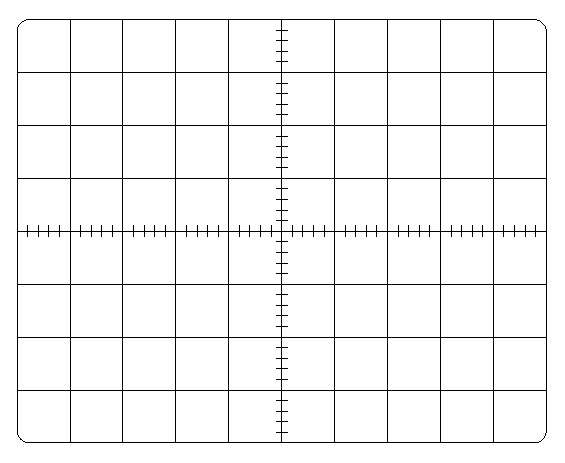
\includegraphics[scale=0.6]{6_induction/scope.eps} & \hspace{1cm} &
\epsfxsize=7cm 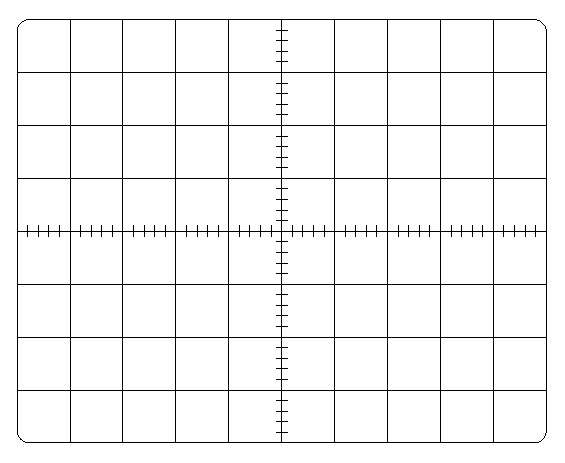
\includegraphics[scale=0.6]{6_induction/scope.eps}
\end{tabular}\\
\ \\

\ \\
\noindent Now set the function generator to produce a good quality square wave
and make a sketch of the input and output signals, on different, labeled
grids, as before. \\
\ \\
\ \\
\begin{tabular}{ccc}
\epsfxsize=7cm 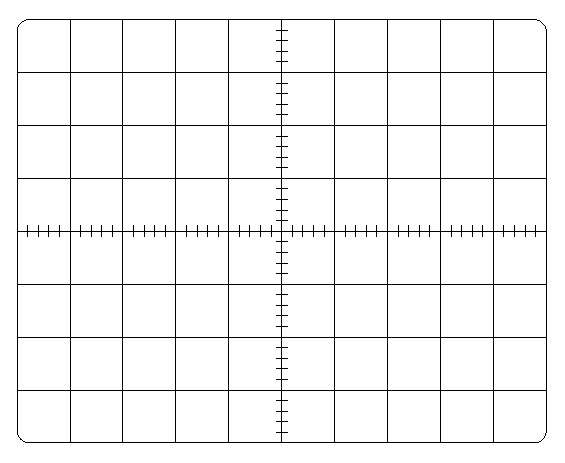
\includegraphics[scale=0.6]{6_induction/scope.eps} & \hspace{1cm} &
\epsfxsize=7cm 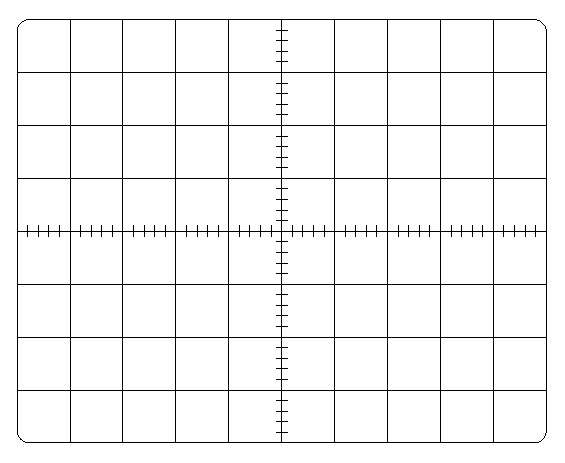
\includegraphics[scale=0.6]{6_induction/scope.eps}
\end{tabular}\\
\ \\





\subsection{Pre-Classroom Check List}
\noindent $\bigcirc$ \hspace*{1cm} Table~\ref{tab:in:Avsw} completed with units and uncertainties \\
$\bigcirc$ \hspace*{1cm} Table~\ref{tab:in:AvsN} completed with units and uncertainties \\
$\bigcirc$ \hspace*{1cm} Sketch of sinusoidal output \\
$\bigcirc$ \hspace*{1cm} Sketch of triangular output \\
$\bigcirc$ \hspace*{1cm} Sketch of square output \\
$\bigcirc$ \hspace*{1cm} Plot and fit of $A_{\rm{out}}/A_{\rm{in}}$ versus
$\omega$ \\
$\bigcirc$ \hspace*{1cm} Plot and fit of $A_{\rm{out}}$ versus N$_2$ \\
$\bigcirc$ \hspace*{1cm} Each student has her/his own plots and worksheet \\
 

\subsection{In-Classroom Calculations $\&$ Discussions}
\subsubsection{Sinusoidal Input}
\noindent {\it The following questions are based on the first sketch,
the sinusoidal output}. Answer the questions completely by  stating your 
reasoning
behind your answers and sketching when necessary. 

\noindent Prove (or disprove) that the output resembles the 
negative of the time derivative of 
the input by comparing the input and output at specific angles and 
showing your reasoning in mathematical terms. Make sure you verify the 
minus sign that appears in Faraday's Law. \\
\vspace*{7cm} \\
\noindent Are there any other characteristics of 
your sketch that help you make an interpretation? \\
\vspace*{3cm} \\

\vfill
\noindent Calculate the phase difference between the input and output 
signals with 
uncertainty (refer to section~\ref{sec:SCOPE:waveprop}). {\bf Show your work}.\\ 
\vspace*{4cm}\\
\hspace*{2cm} {$\phi$ =~\rule{3cm}{.1mm}}\\ 
\noindent What is the phase difference predicted by Faraday's law? Explain your answer.\\
\vspace*{2.5cm} \\

\noindent Compare the calculated phase difference to the predicted phase difference. \\
\vspace*{2cm} \\
\noindent How do the two plots you made (amplitude ratio versus frequency and
output amplitude versus number of turns) agree with Faraday's Law?  
{\bf Be specific and use the law as a guide}.

\vfill 
\pagebreak

\subsubsection{Triangle and Square Wave Input}
\noindent {\it The following questions are based on the sketch of 
the triangular input}. Answer the questions completely by  stating your 
reasoning
behind your answers and sketching when necessary. 
\ \\
\noindent Are the peaks perfectly sharp or do they round off gently, i.e.
how good of a triangular wave are you studying? \\
\vspace*{1.5cm} \\
\noindent Compare the output signal with the negative time derivative of the
input carefully in the space provided. \\
\vspace*{5cm} \\

\clearpage
\noindent {\it The following questions are based on the sketch of 
the square input}.
\noindent Are the corners of the waves perfectly sharp, i.e. how good 
of a square wave are you studying? \\
\vspace*{1cm} \\
\vspace*{1cm} \\
\noindent Again, compare the output signal with the negative time derivative
of the input. \\
\vspace*{5cm} \\
\clearpage

\subsection{Conclusion}

Write a {\it brief} (that is, a one or two paragraph) conclusion for
this lab below. In it, you should summarize the physical
principles which were meant to be illustrated in this experiment. You
should also describe the degree to which your data supported these
principles.

\vfill
\noindent Attach plots to the worksheet. \\
\ \\
{\Large End Worksheet} 
% Go back to ordinary section numbering
\renewcommand{\thesection}{\thechapter.\arabic{section}}














